\subsection{Graphical Spread Results}
\label{subsection:spreadresults}
\subsubsection{Atlantic}
\label{subsubsection:spreadresultsAtlantic}

We look to confirm the results of section \ref{subsubsection:gradientresultsAtlantic}. From analysis of $R_\rho$ and $c$ in this location we expect there to be a surface which is better aligned with the true mixing direction than the neutral surface. The gradient ratios suggest that the ``spread" will be reduced for both $\theta$ and $S$ on the $\sigma_2$ and $\sigma_4$ surfaces, which the smallest ``spread" on $\sigma_4$.

Figures \ref{fig:atlantic_theta} and \ref{fig:atlantic_S} below clearly show a reduced variance of $\theta$ and $S$ on the surfaces $\sigma_2$ and $\sigma_4$ as compared to the neutral surface $\gamma_n$, as we expect. It also shows that $\sigma_4$, given in figures \ref{fig:subplot_atlantic_theta_sig4} and \ref{fig:subplot_atlantic_S_sig4} has the smallest ``spread" and is therefore best aligned with the true mixing direction, as predicted by the mathematical theory. 

\begin{figure}[htbp]
    \centering
    \begin{subfigure}[b]{0.4\textwidth}
         \centering
         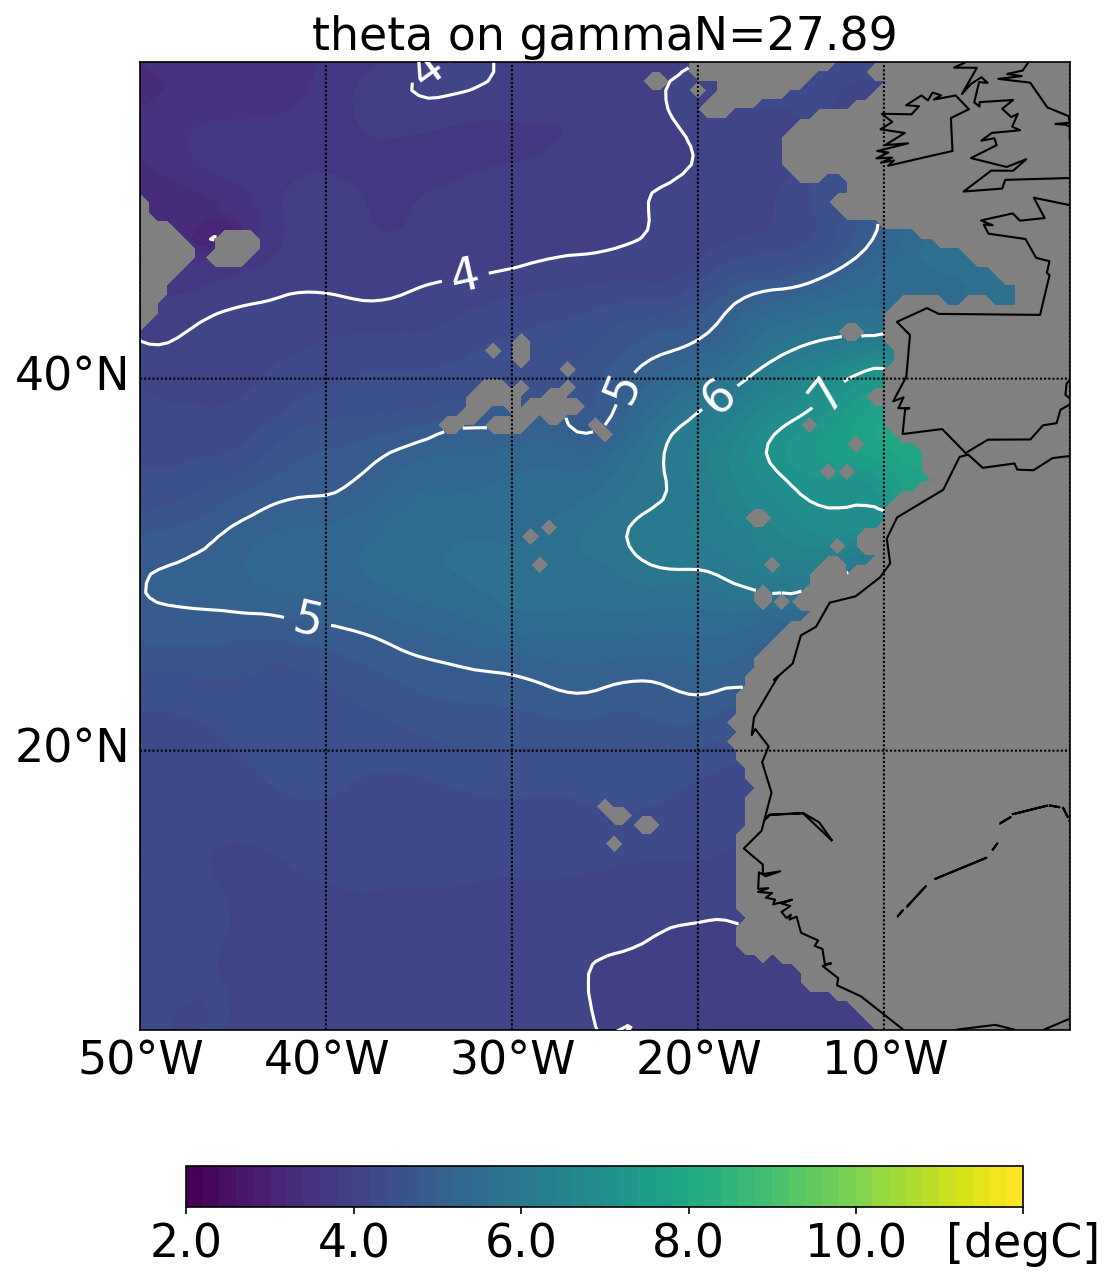
\includegraphics[width=\textwidth]{atlantic_theta/Map2dcyl_theta_on_gammaN_2789e-2_reg310Eto360E05Nto57N_1990to1998av_WOCE}
         \caption{$\gamma_n = 28.89$}
         \label{fig:subplot_atlantic_theta_gammaN}
     \end{subfigure}
     \hfill
     \begin{subfigure}[b]{0.4\textwidth}
         \centering
         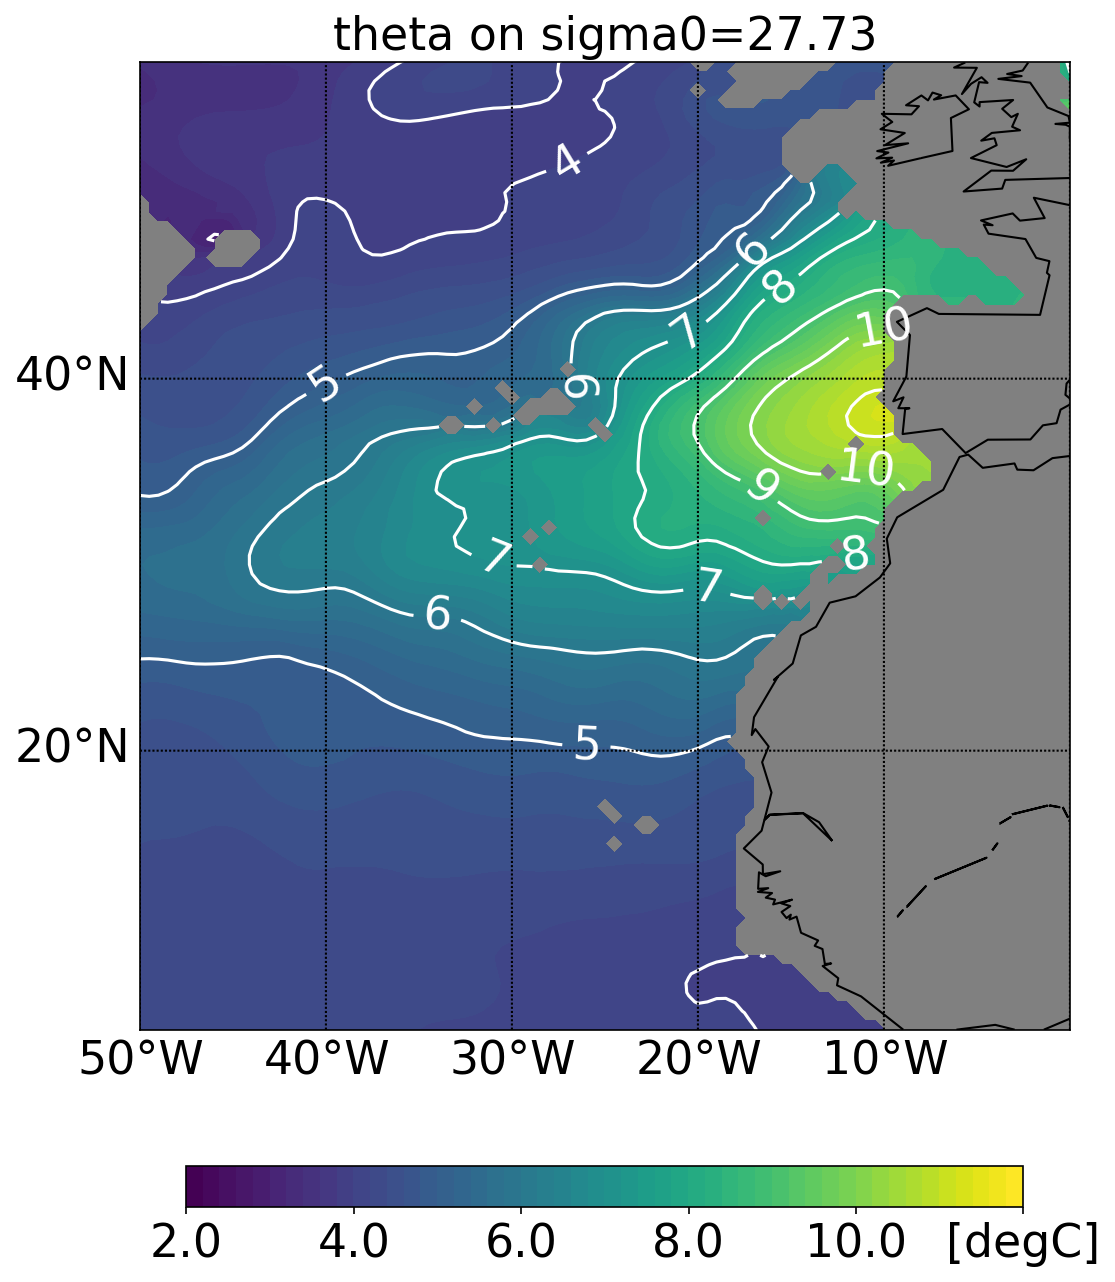
\includegraphics[width=\textwidth]{atlantic_theta/Map2dcyl_theta_on_sigma0_2773e-2_reg310Eto360E05Nto57N_1990to1998av_WOCE}
         \caption{$\sigma_0 = 27.73$}
         \label{fig:subplot_atlantic_theta_sig0}
     \end{subfigure}
     \begin{subfigure}[b]{0.4\textwidth}
         \centering
         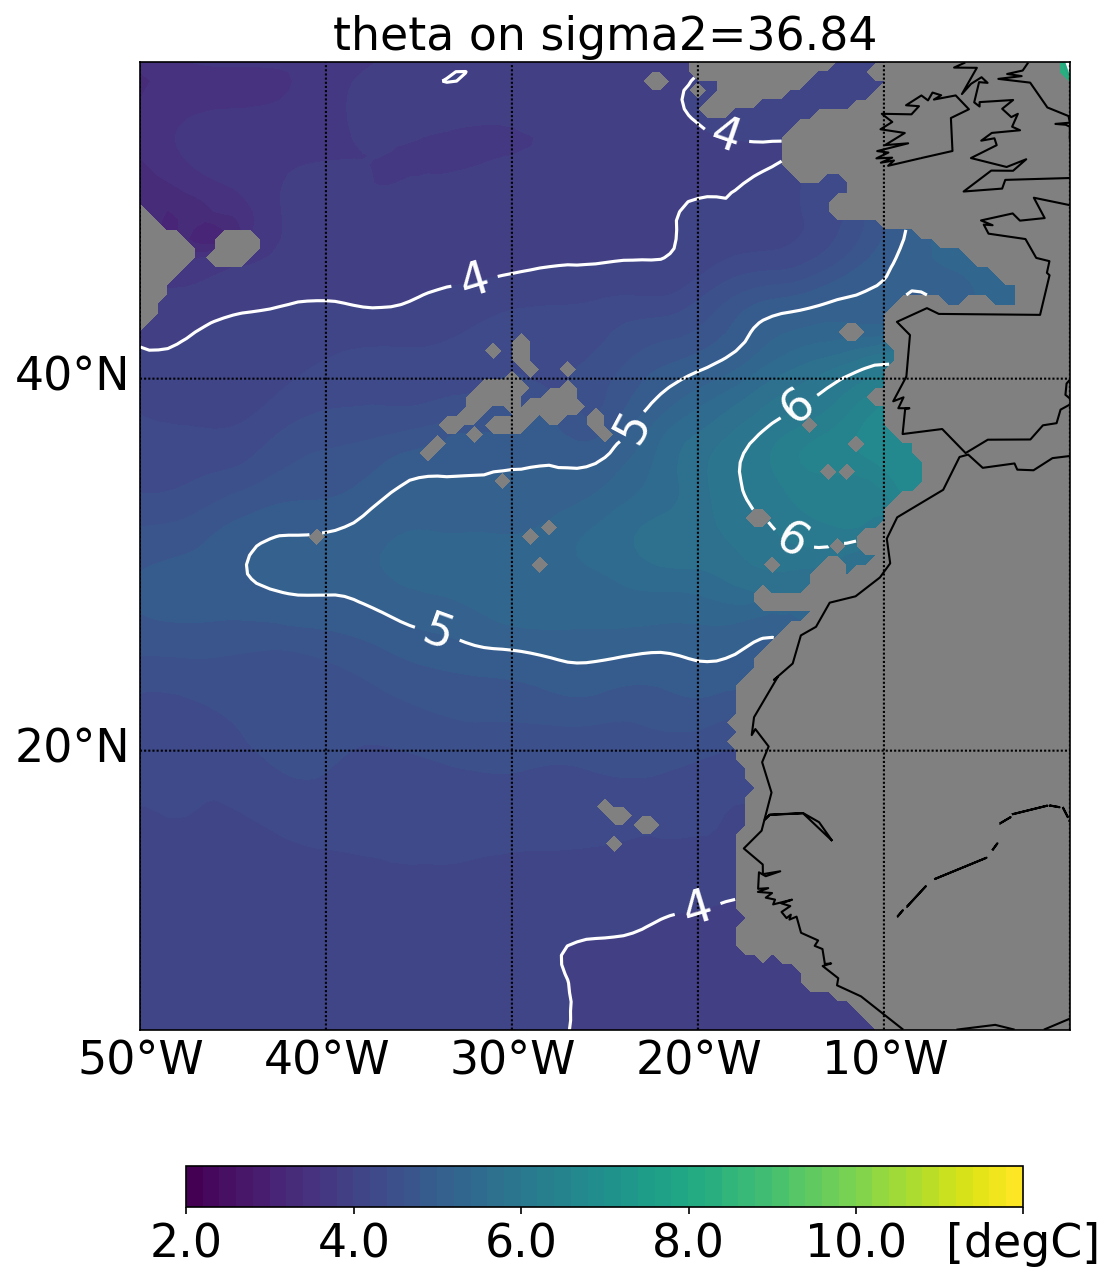
\includegraphics[width=\textwidth]{atlantic_theta/Map2dcyl_theta_on_sigma2_3684e-2_reg310Eto360E05Nto57N_1990to1998av_WOCE}
         \caption{$\sigma_2 = 36.84$}
         \label{fig:subplot_atlantic_theta_sig2}
     \end{subfigure}
     \hfill
     \begin{subfigure}[b]{0.4\textwidth}
         \centering
         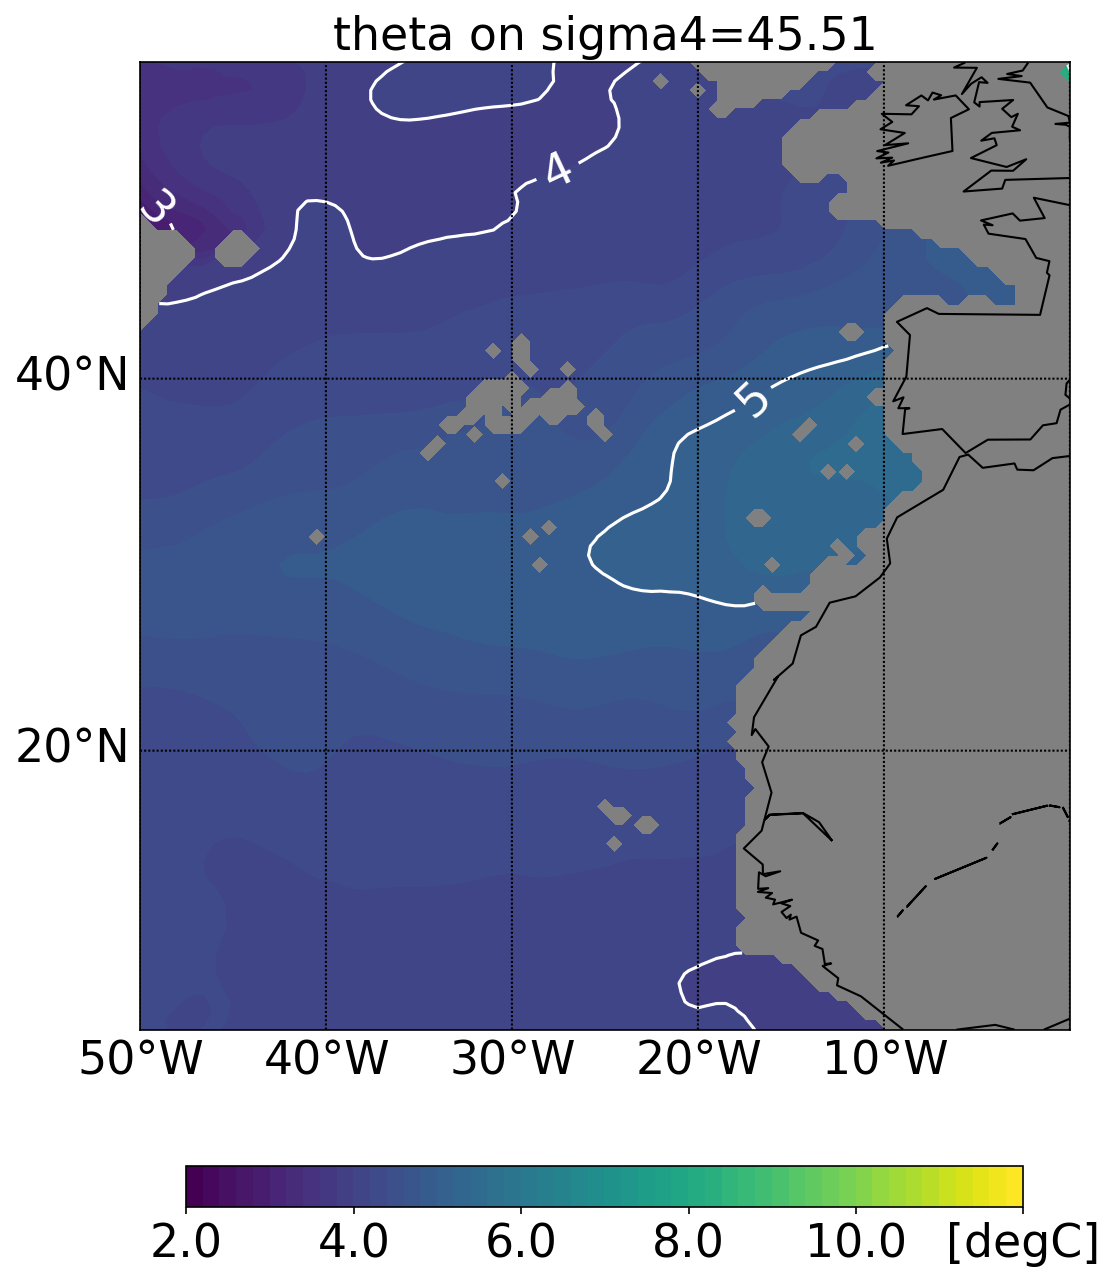
\includegraphics[width=\textwidth]{atlantic_theta/Map2dcyl_theta_on_sigma4_4551e-2_reg310Eto360E05Nto57N_1990to1998av_WOCE}
         \caption{$\sigma_4 = 45.51$}
         \label{fig:subplot_atlantic_theta_sig4}
     \end{subfigure}
    \caption{$\theta$ projected onto the surfaces of interest outlined in section \ref{subsubsection:spreadmethodatlanticocean}}
    \label{fig:atlantic_theta}
    
\end{figure}

\begin{figure}[htbp]
    \centering
     \begin{subfigure}[b]{0.4\textwidth}
         \centering
         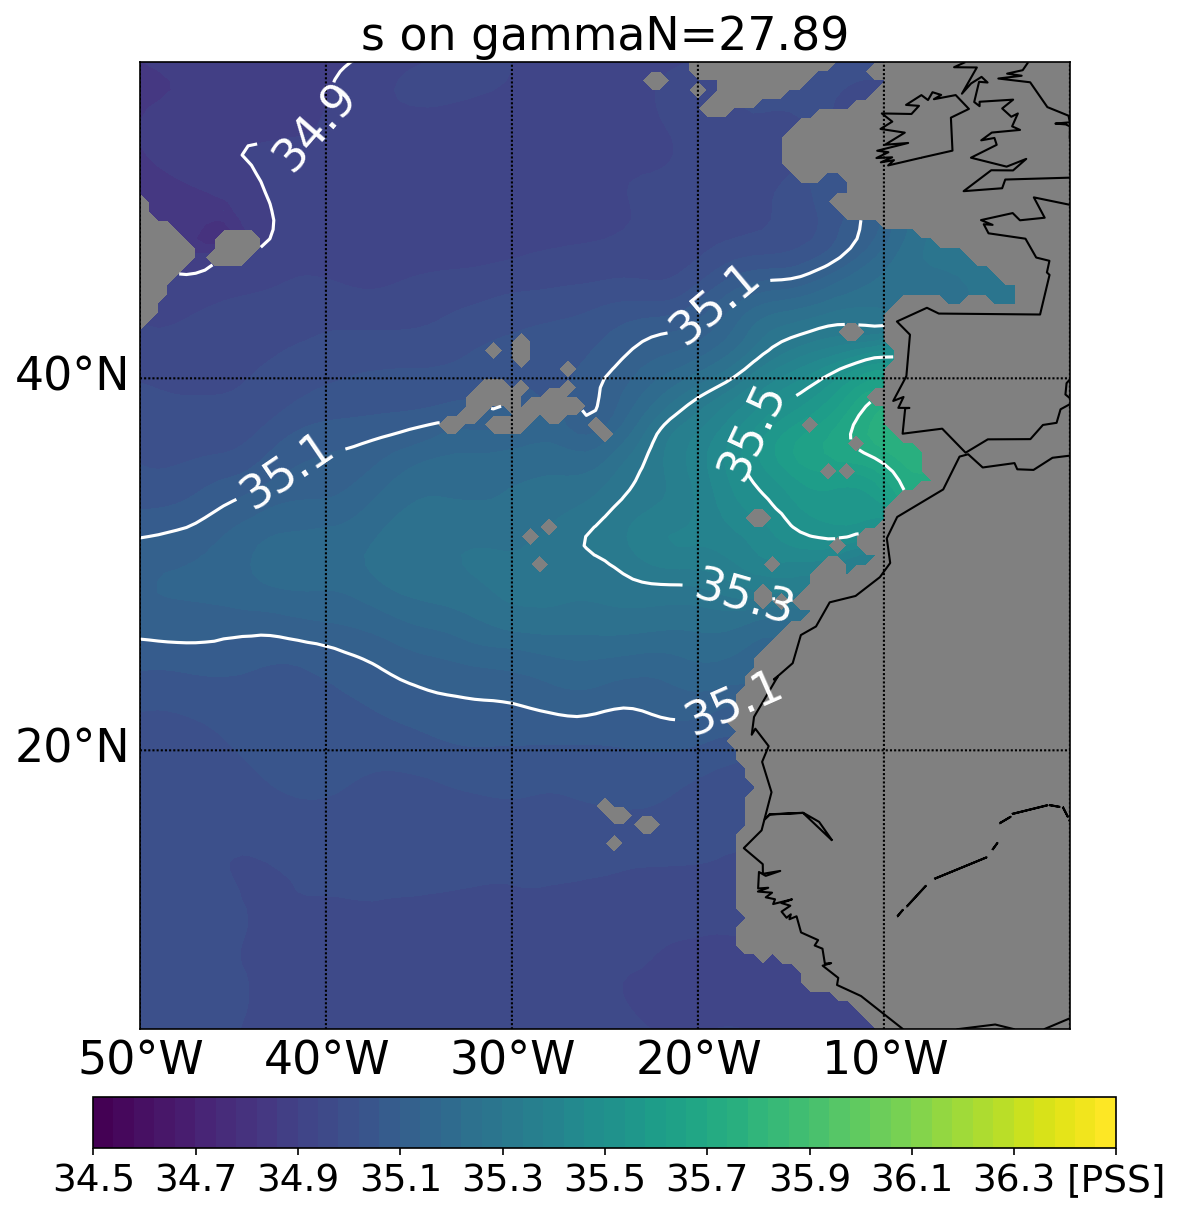
\includegraphics[width=\textwidth]{atlantic_s/Map2dcyl_s_on_gammaN_2789e-2_reg310Eto360E05Nto57N_1990to1998av_WOCE}
         \caption{$\gamma_n = 28.89$}
         \label{fig:subplot_atlantic_S_gammaN}
     \end{subfigure}
     \hfill
     \begin{subfigure}[b]{0.4\textwidth}
         \centering
         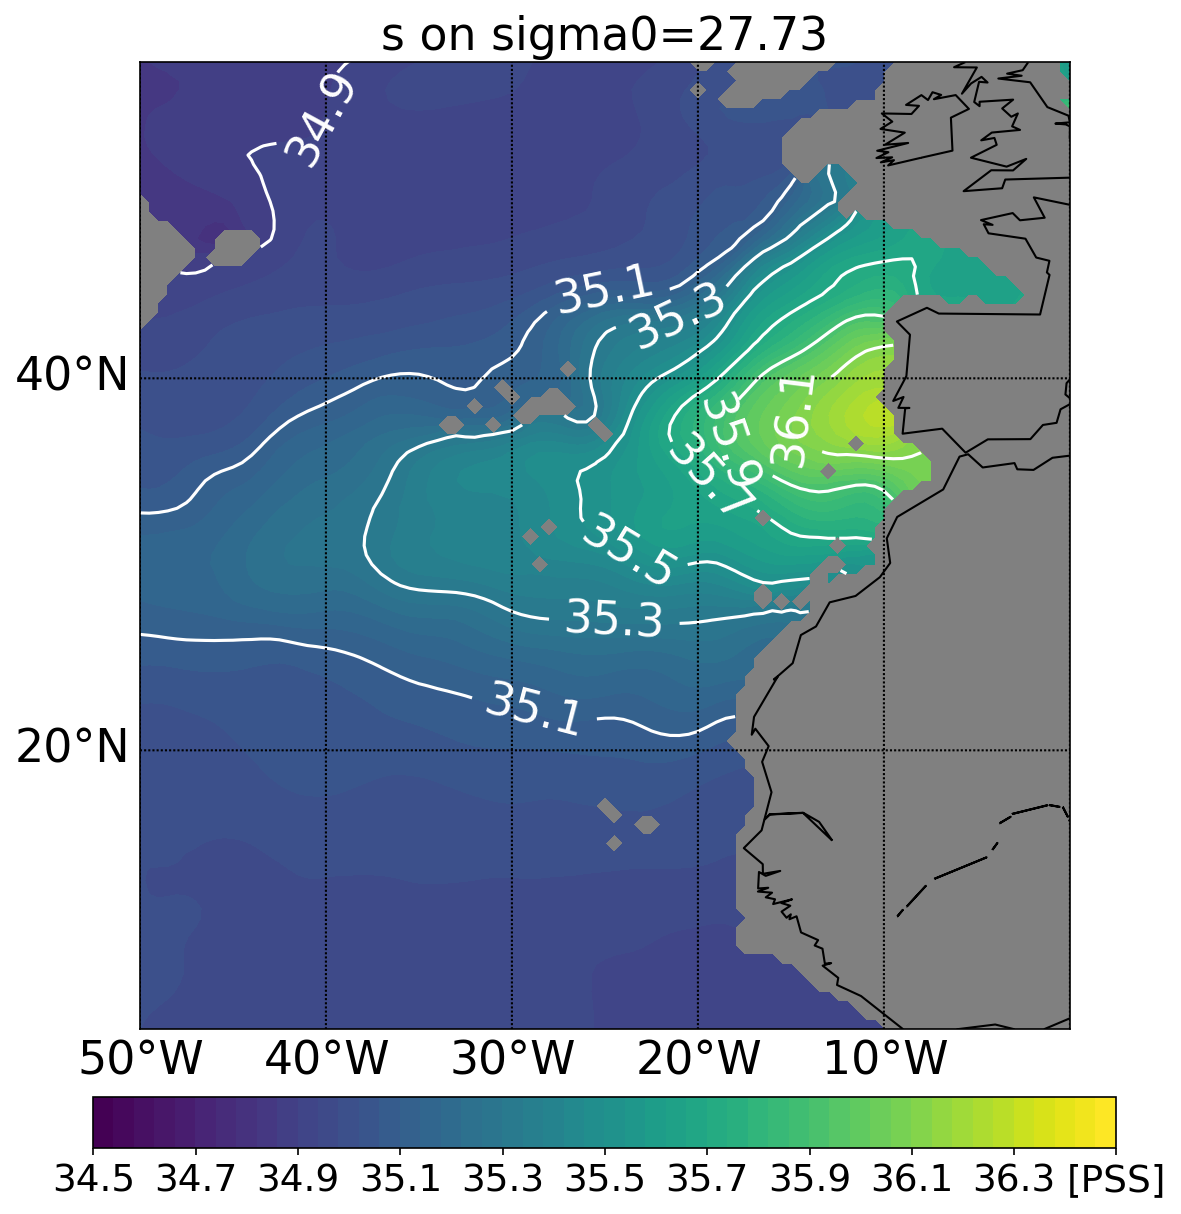
\includegraphics[width=\textwidth]{atlantic_s/Map2dcyl_s_on_sigma0_2773e-2_reg310Eto360E05Nto57N_1990to1998av_WOCE}
         \caption{$\sigma_0 = 27.73$}
         \label{fig:subplot_atlantic_S_sig0}
     \end{subfigure}
    \begin{subfigure}[b]{0.4\textwidth}
         \centering
         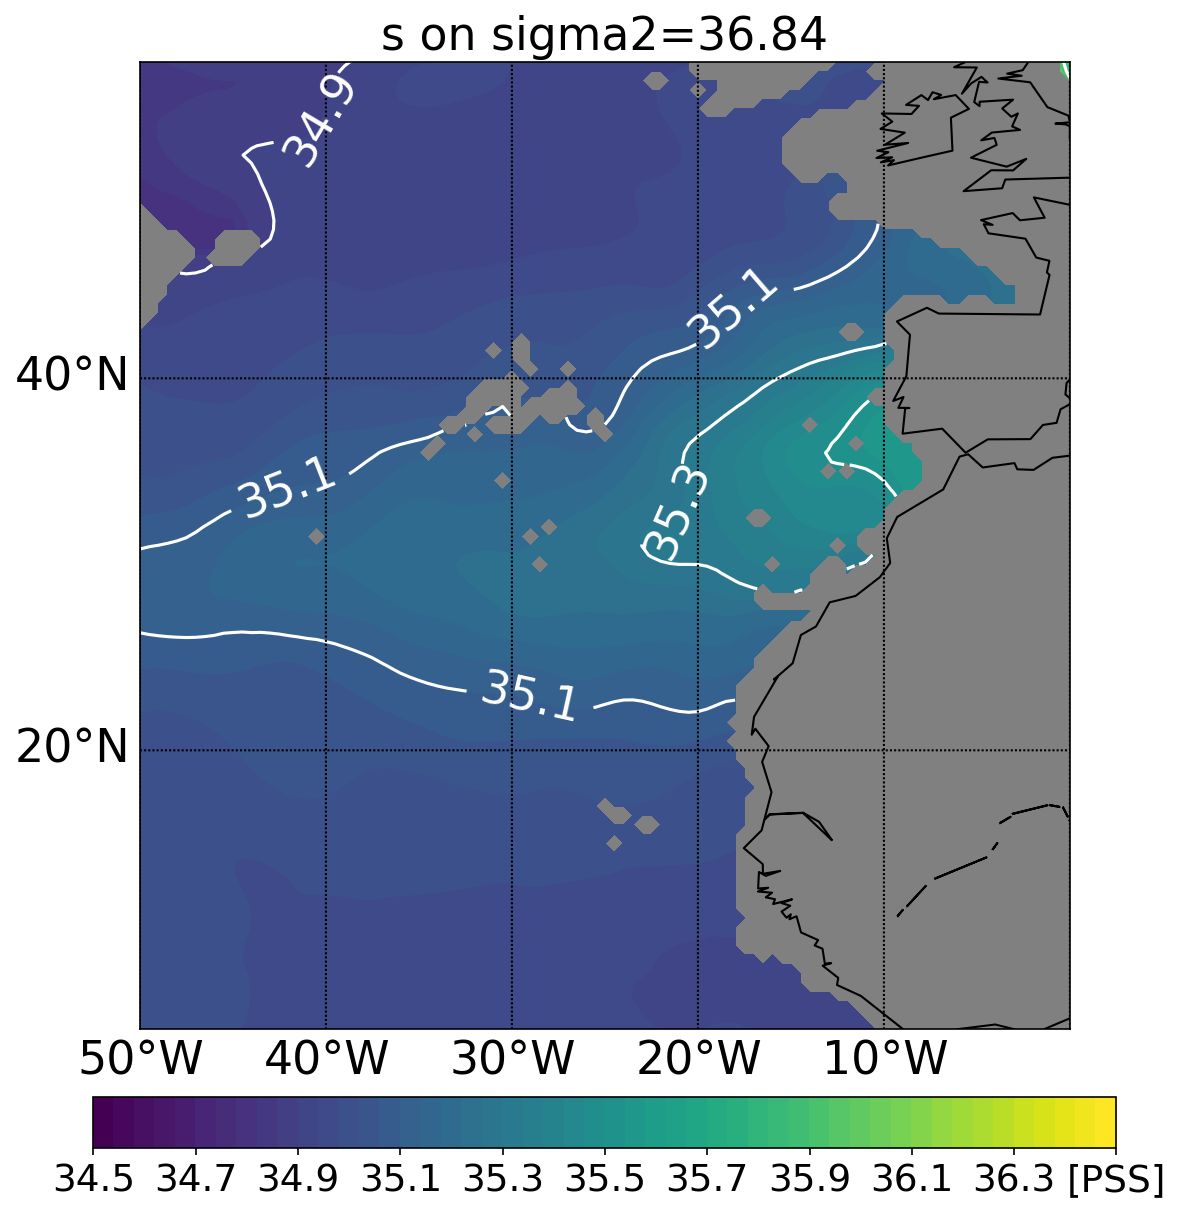
\includegraphics[width=\textwidth]{atlantic_s/Map2dcyl_s_on_sigma2_3684e-2_reg310Eto360E05Nto57N_1990to1998av_WOCE}
         \caption{$\sigma_2 = 36.84$}
         \label{fig:subplot_atlantic_S_sig2}
     \end{subfigure}
     \hfill
     \begin{subfigure}[b]{0.4\textwidth}
         \centering
         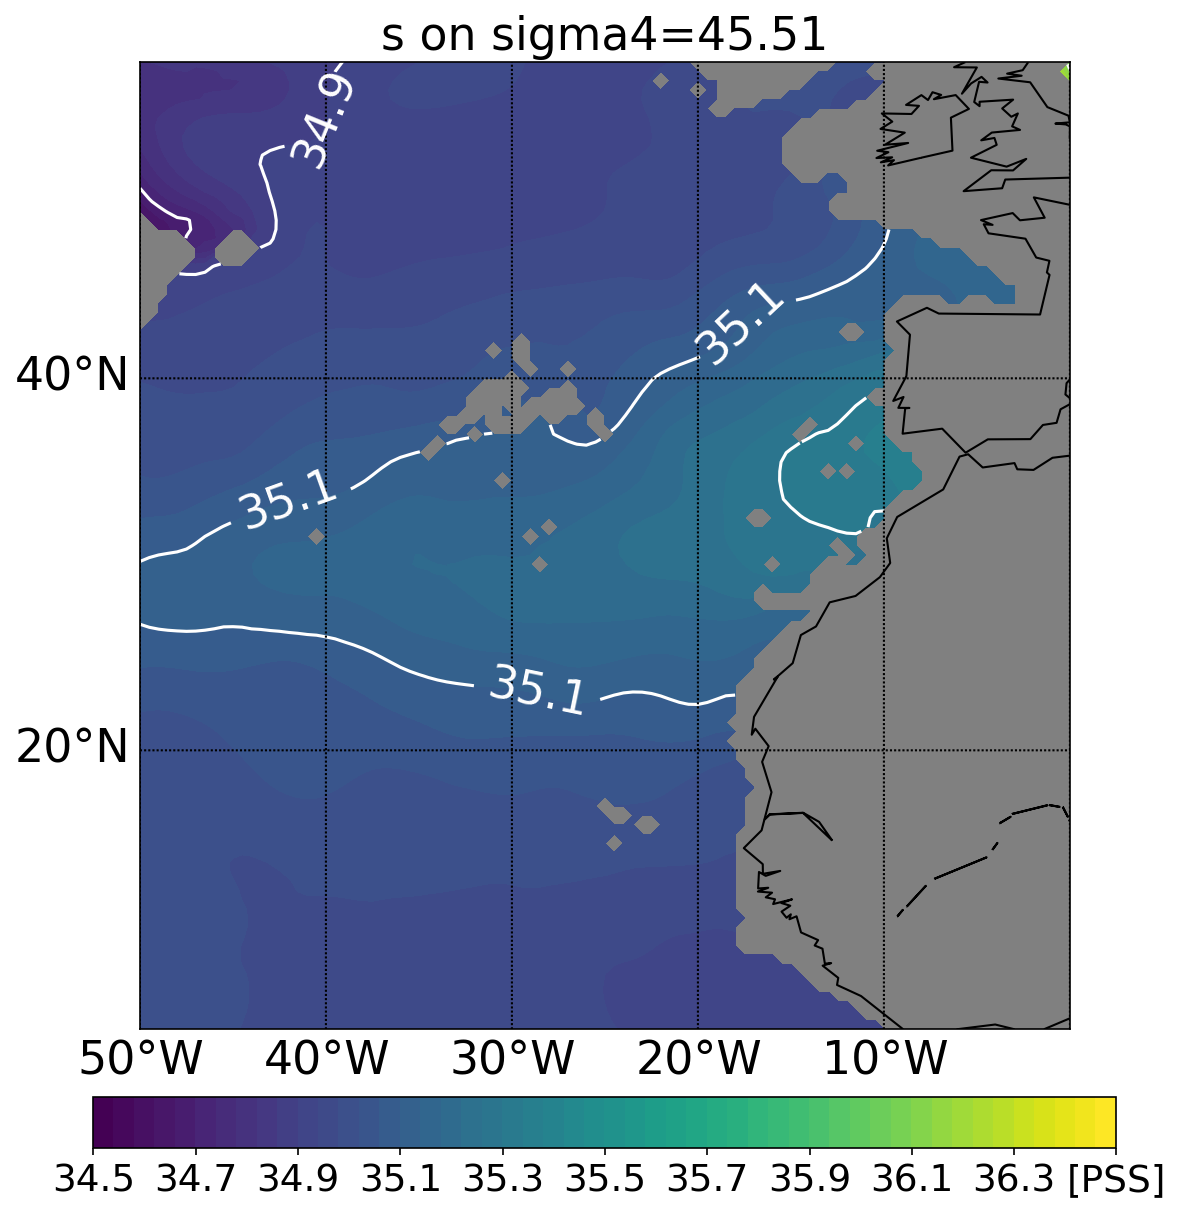
\includegraphics[width=\textwidth]{atlantic_s/Map2dcyl_s_on_sigma4_4551e-2_reg310Eto360E05Nto57N_1990to1998av_WOCE}
         \caption{$\sigma_4 = 45.51$}
         \label{fig:subplot_atlantic_S_sig4}
     \end{subfigure}
    \caption{$S$ projected onto the surfaces of interest outlined in section \ref{subsubsection:spreadmethodatlanticocean}}
    \label{fig:atlantic_S}
\end{figure}

\subsubsection{Gibraltar Strait}
\label{subsubsection:spreadresultsgibraltar}

From the mathematical analysis performed in section \ref{subsection:gradienttresults} we are expecting to see a reduced ``spread" for $\theta$ on the $\sigma_2$ and $\sigma_4$ surfaces when compared to the neutral surface. We also expect the spread to be larger on $\sigma_0$. This is reflected in figure \ref{fig:gibraltar_theta}.

The picture for $S$ is more complicated; the analysis from the previous section suggested that there may be a section of reduced ``spread" and a section of increased ``spread" for $S$ on the potential density surfaces when compared to the $\gamma_n$ surface. This is perhaps clearest on the $\sigma_0$ surface shown in figure \ref{fig:subplot_gibraltar_S_sig0}. 

Close to the source region at the Gibraltar Straight the contours on the $\sigma_0$ are closer together than the contours on the $\gamma_n$ surface (figure \ref{fig:subplot_gibraltar_S_gammaN}) suggesting an increased ``spread" and hence a higher gradient. However in the region below $25^{\circ}$N the contours are much more widely spaced, suggesting a reduced gradient in that region. This aligns with the gradient ratio shown in figure \ref{fig:subplot_atlantic_grad_s_sig0} in the previous section. 

\begin{figure}[htbp]
    \centering
    \begin{subfigure}[b]{0.4\textwidth}
         \centering
         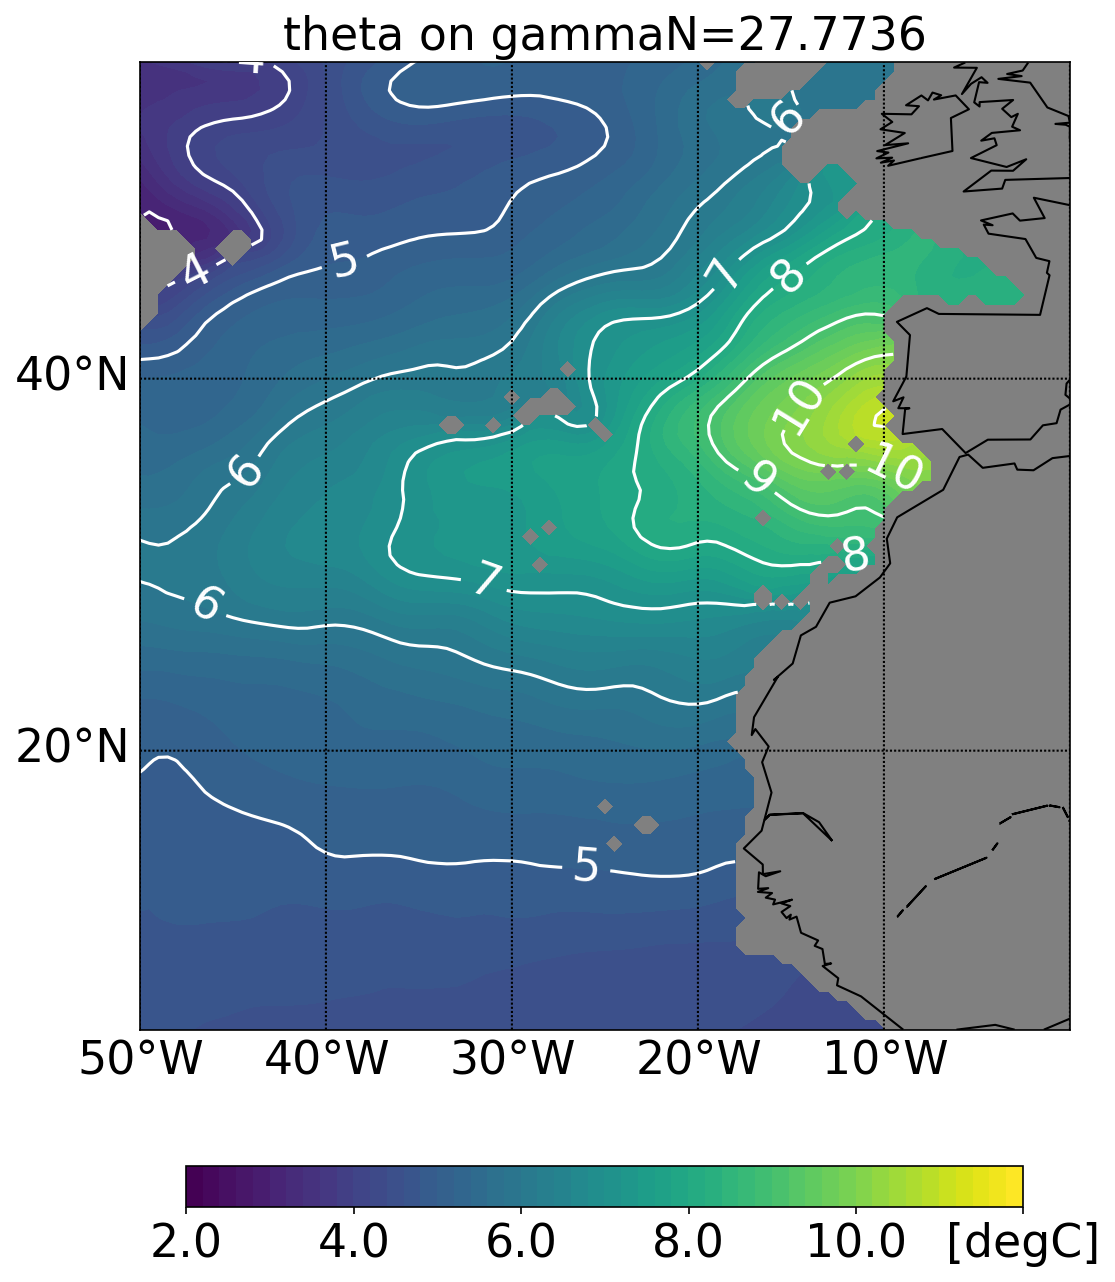
\includegraphics[width=\textwidth]{gibraltar_theta/Map2dcyl_theta_on_gammaN_2777e-2_reg310Eto360E05Nto57N_1990to1998av_WOCE}
         \caption{$\gamma_n = 27.7736$}
         \label{fig:subplot_gibraltar_theta_gammaN}
     \end{subfigure}
     \hfill
     \begin{subfigure}[b]{0.4\textwidth}
         \centering
         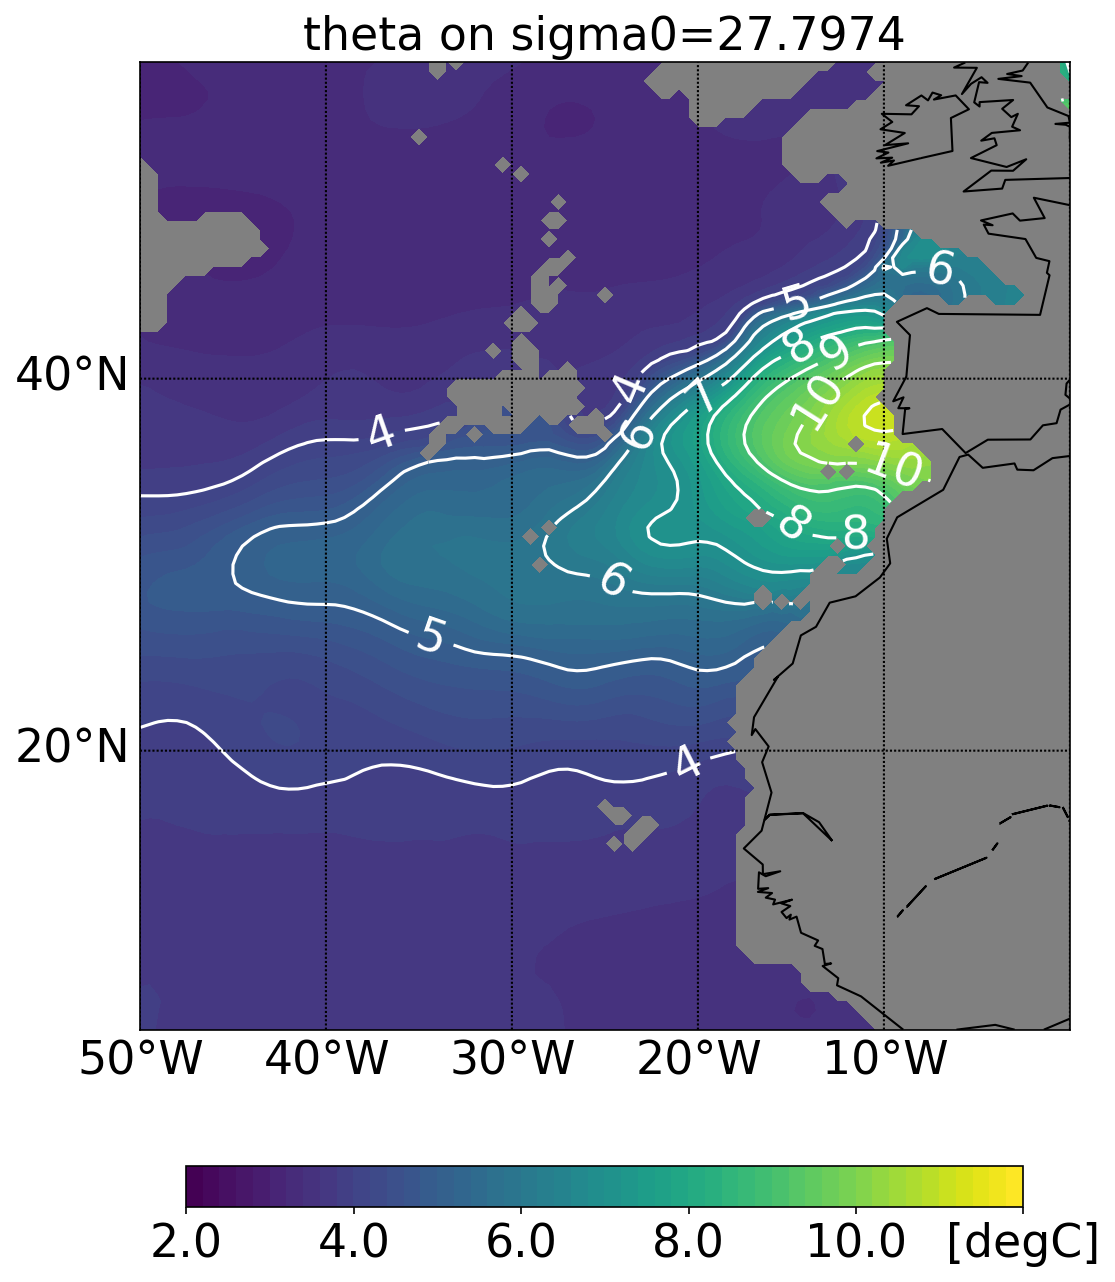
\includegraphics[width=\textwidth]{gibraltar_theta/Map2dcyl_theta_on_sigma0_2779e-2_reg310Eto360E05Nto57N_1990to1998av_WOCE}
         \caption{$\sigma_0 = 27.7974$}
         \label{fig:subplot_gibraltar_theta_sig0}
     \end{subfigure}
     \begin{subfigure}[b]{0.4\textwidth}
         \centering
         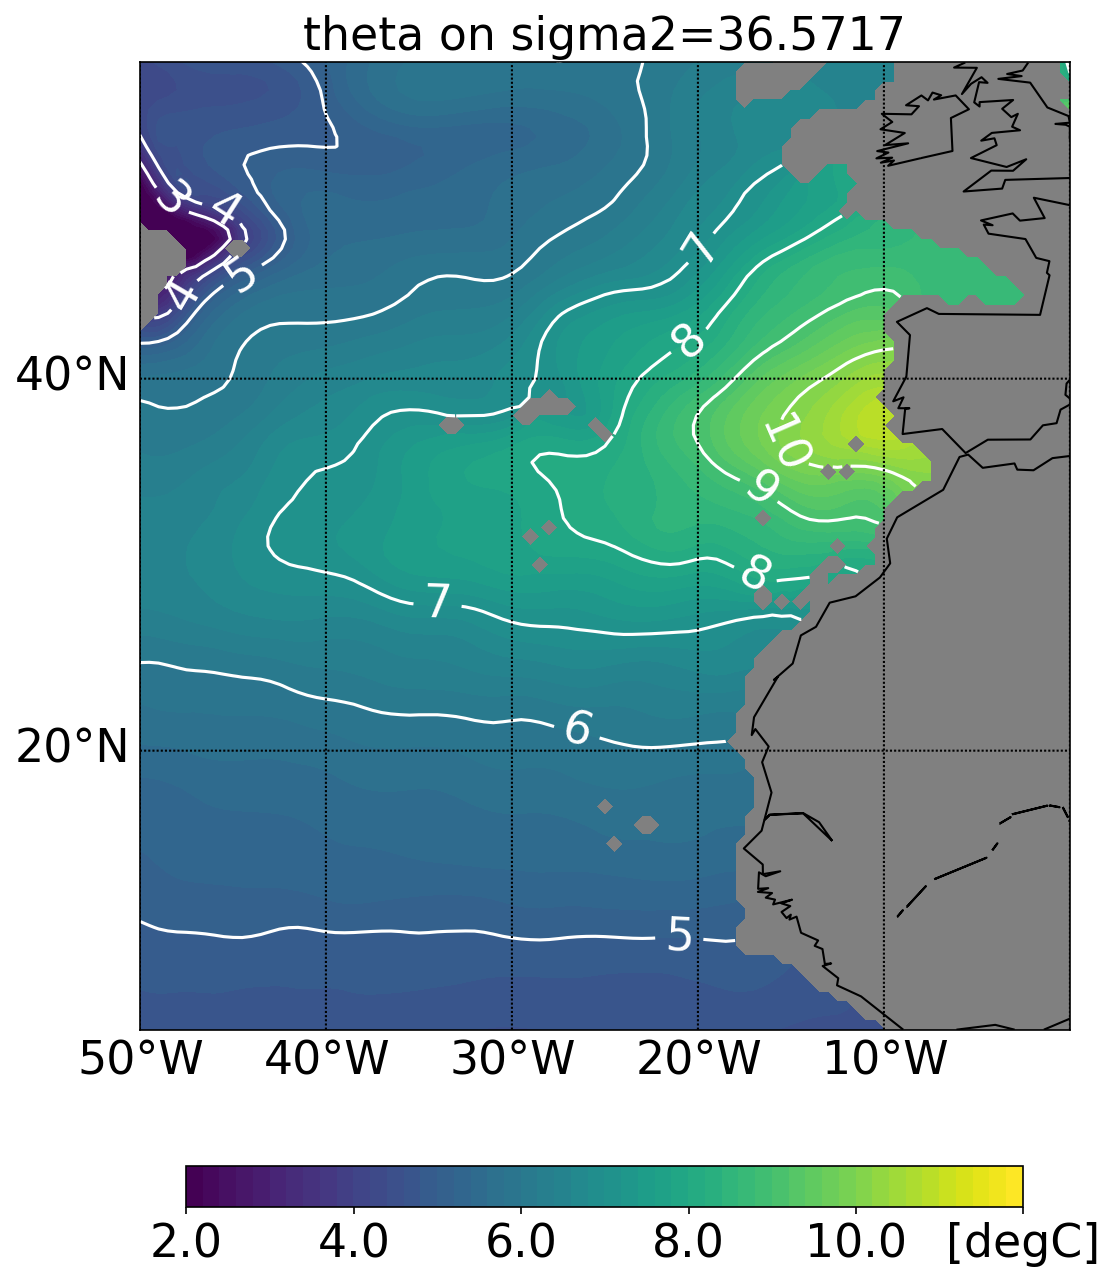
\includegraphics[width=\textwidth]{gibraltar_theta/Map2dcyl_theta_on_sigma2_3657e-2_reg310Eto360E05Nto57N_1990to1998av_WOCE}
         \caption{$\sigma_2 = 36.5717$}
         \label{fig:subplot_gibraltar_theta_sig2}
     \end{subfigure}
     \hfill
     \begin{subfigure}[b]{0.4\textwidth}
         \centering
         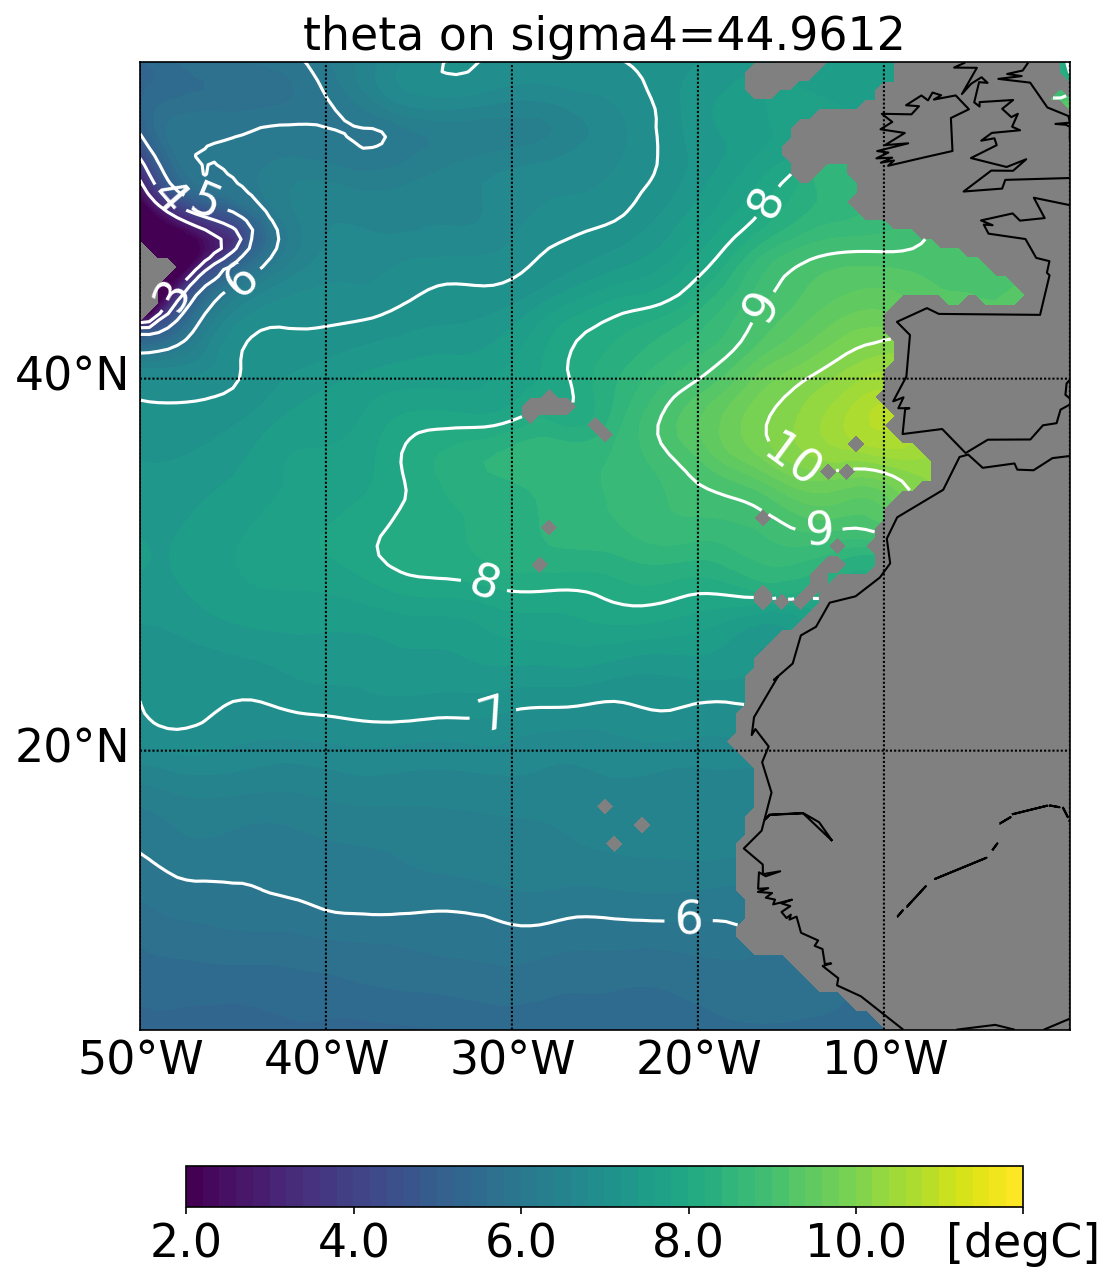
\includegraphics[width=\textwidth]{gibraltar_theta/Map2dcyl_theta_on_sigma4_4496e-2_reg310Eto360E05Nto57N_1990to1998av_WOCE}
         \caption{$\sigma_4 = 44.9612$}
         \label{fig:subplot_gibraltar_theta_sig4}
     \end{subfigure}
    \caption{$\theta$ projected onto the surfaces of interest outlined in section \ref{subsubsection:spreadmethodgibraltarstraight}}
    \label{fig:gibraltar_theta}
    
\end{figure}

\begin{figure}[htbp]
    \centering
     \begin{subfigure}[b]{0.4\textwidth}
         \centering
         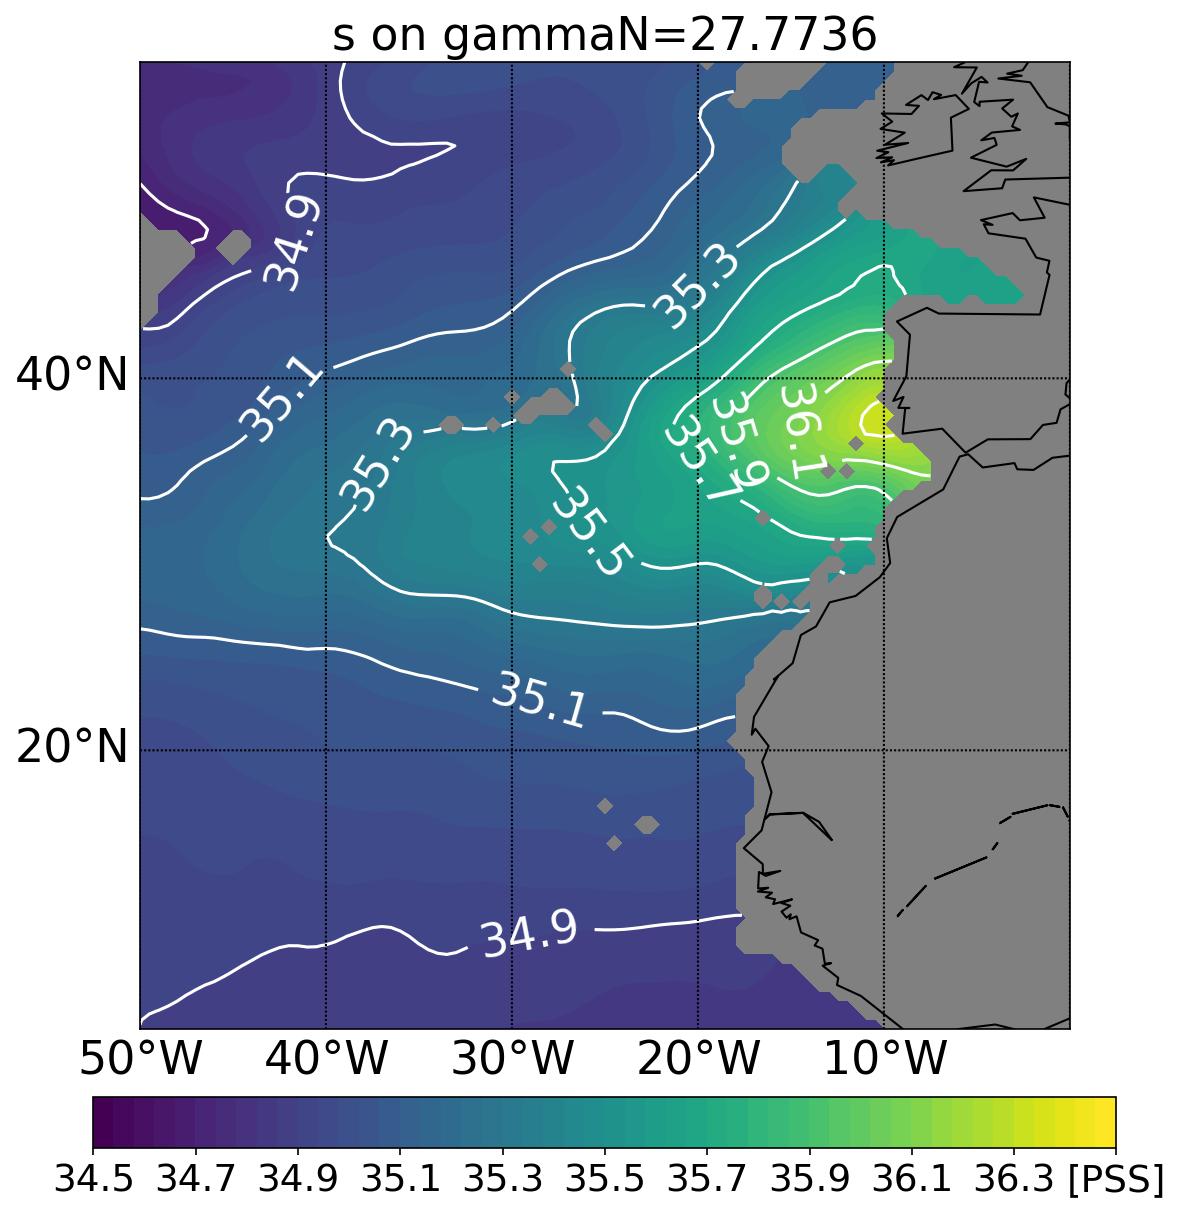
\includegraphics[width=\textwidth]{gibraltar_s/Map2dcyl_s_on_gammaN_2777e-2_reg310Eto360E05Nto57N_1990to1998av_WOCE}
         \caption{$\gamma_n = 27.7736$}
         \label{fig:subplot_gibraltar_S_gammaN}
     \end{subfigure}
     \hfill
     \begin{subfigure}[b]{0.4\textwidth}
         \centering
         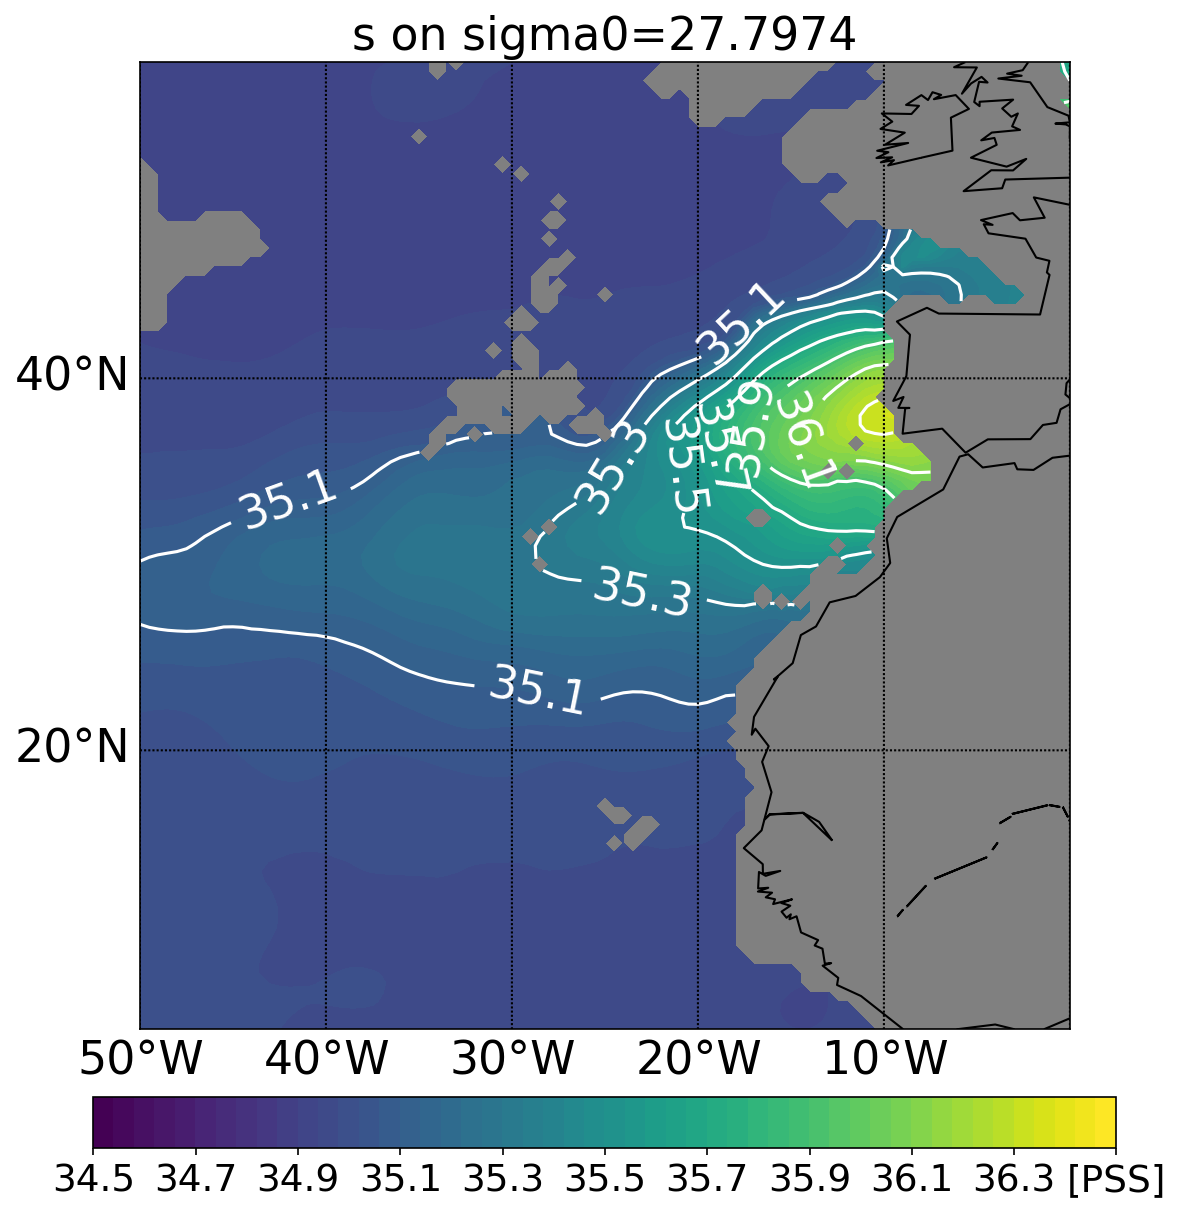
\includegraphics[width=\textwidth]{gibraltar_s/Map2dcyl_s_on_sigma0_2779e-2_reg310Eto360E05Nto57N_1990to1998av_WOCE}
         \caption{$\sigma_0 = 27.7974$}
         \label{fig:subplot_gibraltar_S_sig0}
     \end{subfigure}
    \begin{subfigure}[b]{0.4\textwidth}
         \centering
         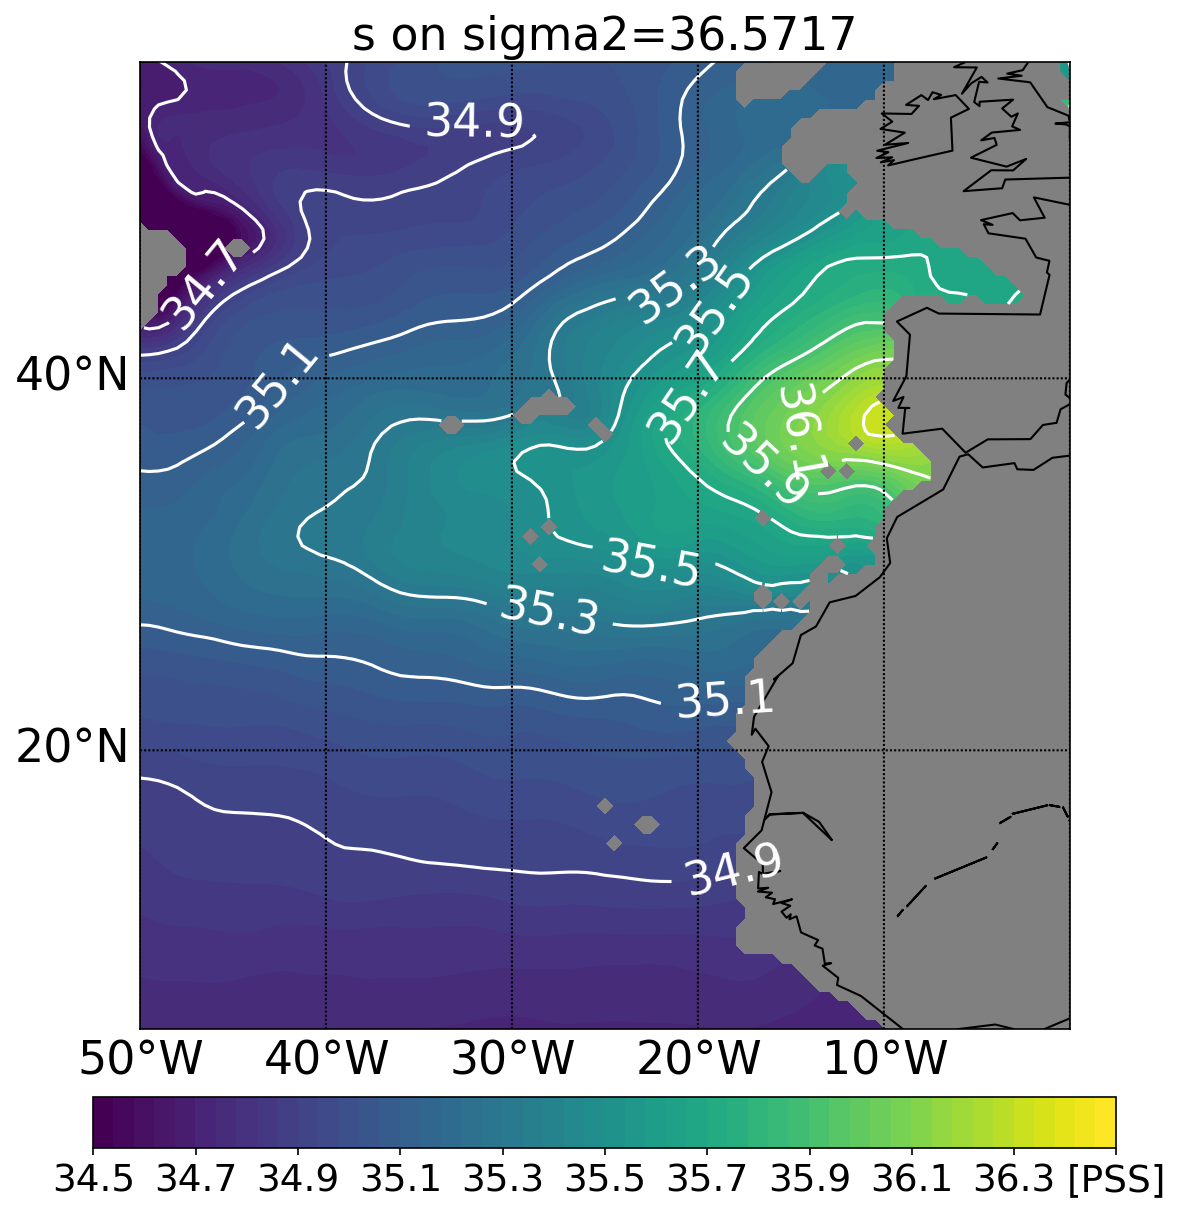
\includegraphics[width=\textwidth]{gibraltar_s/Map2dcyl_s_on_sigma2_3657e-2_reg310Eto360E05Nto57N_1990to1998av_WOCE}
         \caption{$\sigma_2 = 36.5717$}
         \label{fig:subplot_gibraltar_S_sig2}
     \end{subfigure}
     \hfill
     \begin{subfigure}[b]{0.4\textwidth}
         \centering
         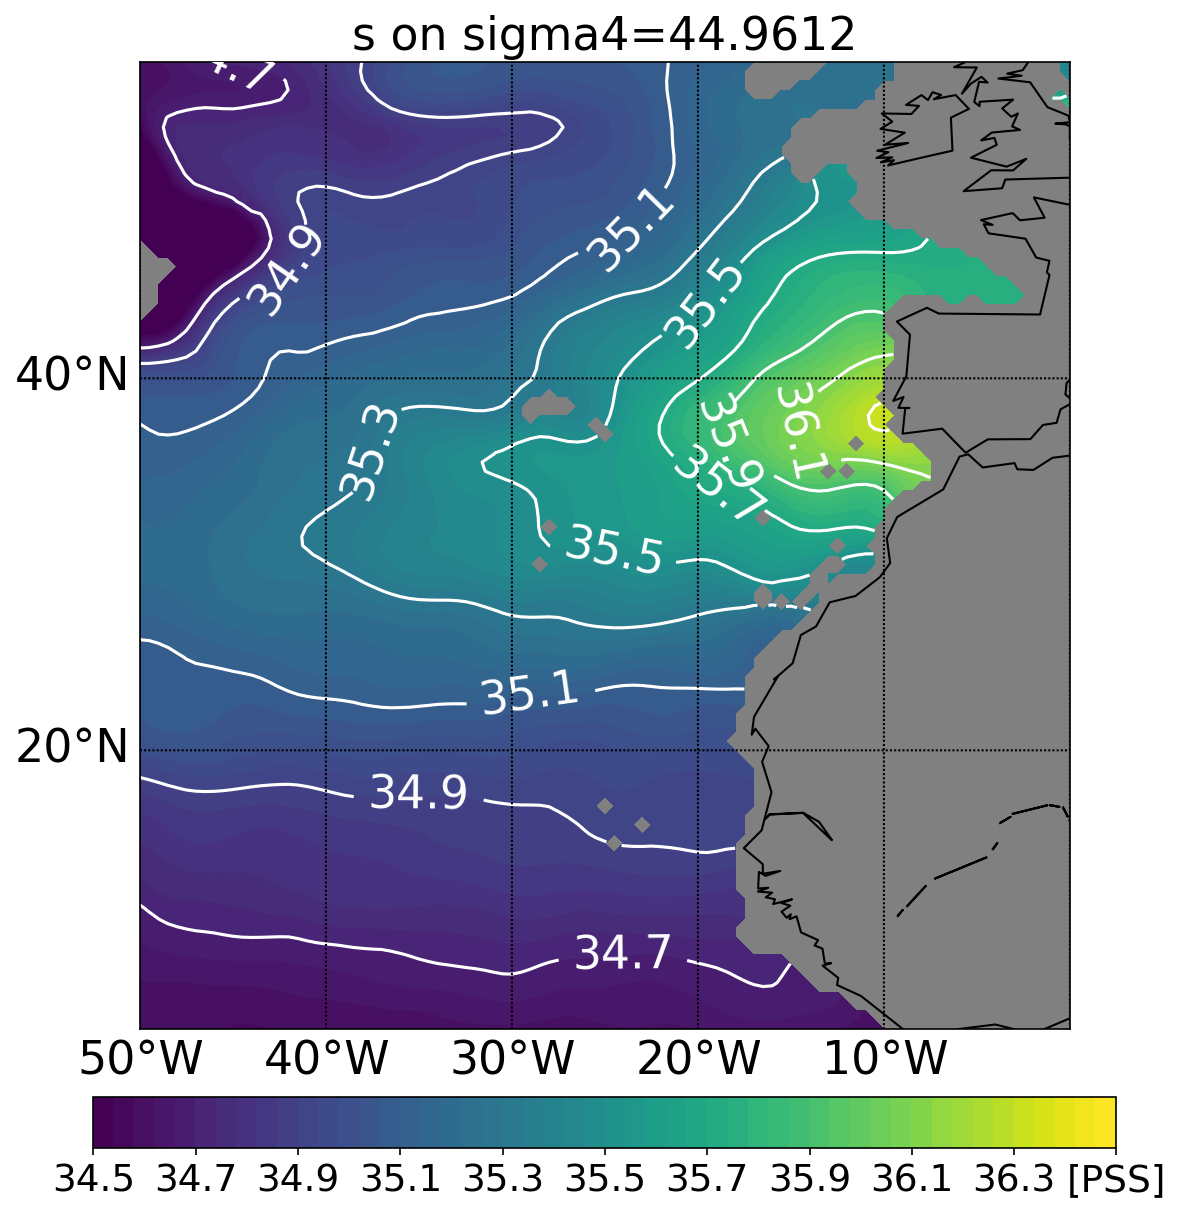
\includegraphics[width=\textwidth]{gibraltar_s/Map2dcyl_s_on_sigma4_4496e-2_reg310Eto360E05Nto57N_1990to1998av_WOCE}
         \caption{$\sigma_4 = 44.9612$}
         \label{fig:subplot_gibraltar_S_sig4}
     \end{subfigure}
    \caption{$S$ projected onto the surfaces of interest outlined in section \ref{subsubsection:spreadmethodgibraltarstraight}}
    \label{fig:gibraltar_S}
\end{figure}

In general what we can see from the plots given in this section is that there is a very clear relationship between the mathematical gradient ratios expressed in section \ref{section:gradienttheorymathematical} and physical spread of a variable along a given surface. The real ocean does behave as we expect using the mathematical tools given in \citet{McDougall1987}. 

This section also clearly shows that if the criteria for selecting a mixing surface is that it minimises the gradient of $\theta$ and $S$ that the neutral surface is not always the correct surface: $\sigma_4$ is a good alternative candidate. 